\myparagraph{Purpose}
Any third party who wants to subscribe to \textit{Data4Help} must go through the registration process, which can be carried out through \textit{Data4Help} web site. The process requires several mandatory steps:
\begin{enumerate}
  \item The third party which aim to become a new member is required to fill in all the fields in which it is asked for information about the company itself like: its business name, its VAT number, its legal address, its billing address, its corporate e-mail address and the sector in which it operates;
  \item The third party must also provide the data of its legal representative, in particular his/her name, his/her surname, his/her office address, his/her phone number, his/her e-mail address and his/her SSN;
  \item The third party must accept different conditions:
    \begin{itemize}
      \item It must assume responsibility in case of unauthorized disclosure of user data;
      \item It must accept Milan as the place of jurisdiction in the case of a legal dispute.
    \end{itemize}
\end{enumerate}
After that the system will check the correctness of the inserted data, in particular it will check that the third party isn't already registered. If the result of this control is positive the registration is authorized and the third party will receive a confirmation e-mail to the specified e-mail address with the password it has to use to access to \textit{Data4Help} services.
From now we will refer to the third party that wants to become a new member as "\textbf{Special user to Be}" to distinguish it from an Individual user.

\myparagraph{Scenario 1}
PharmaAnalisi SPA wants to acquire data of a group of young people in order to do an analysis about the kind of life they conduct. It opens the browser and search for \textit{Data4Help} web site, then it clicks on the "\textit{Third Party Sign In}" button, which is located in the main page. It passes through the steps of the registration process, inserting all the required data but forgotting to accept one of the conditions. As a consequence the system won't permit it to conclude the registration process, so it checks again and figures out what was missing, it accepts the condition and submits its registration. Finally, it receives the confimation e-mail.

\myparagraph{Use Case}
The \textit{Third Party Sign In} use case is analyzed in Table \ref{table:thirdPartySignInTable}.

\myparagraph{Activity Diagram}
The \textit{Third Party Sign In} activity diagram is shown in Figure \ref{img:specialSignInActivityDiagram}.

\myparagraph{Mockup}
The \textit{Third Party Sign In} mocukp is shown in Figure \ref{img:thirdPartySignInMockup}.

\myparagraph{Functional requirements}
\begin{enumerate}
  \item The system must not accept an e-mail address that is already used by an already registered third party;
  \item The system must not accept a business name that is already used by an already registered third party;
  \item The system must not accept a VAT number that is already used by an already registered third party;
  \item The system must not authorize the registration untill all the fields are filled up;
  \item The system must not authorize the registration untill the required conditions aren't accepted;
  \item The system must send the confirmation e-mail to the inserted e-mail address with the password when "\textit{Submit}" button is clicked only if all the inserted data are acceptable and the required conditions has been accepted;
  \item The system must let the \textbf{Special user to be} leave the registration process at anytime.
\end{enumerate}

\begin{center}
\begin{table}[H]
  \scalebox{0.9}{
\begin{tabular}{ | l | p{0.75\linewidth} | }
  \hline
    Actor & \textbf{Special user to be} \\ \hline
    Goal & \textbf{[G.1]} \\ \hline
    Input Condition & A third party wants to subscribe to \textit{Data4Help} services \\ \hline
    Event Flow & \begin{minipage}[t]{0.7\textwidth}
      \begin{enumerate}
        \item The \textbf{Special user to be} opens the main page of \textit{Data4Help} web site.
        \item The \textbf{Special user to be} clicks on "\textit{Sign in (Third party)}" button;
        \item The system shows the form the \textbf{Special user to be} has to fill up;
        \item The \textbf{Special user to be} fills up the form with its business name, its VAT number, its legal address, its billing address, its corporate e-mail address and the sector in which it operates;
        \item The \textbf{Special user to be} accepts the required conditions;
        \item The \textbf{Special user to be} clicks on "\textit{Submit}" button;
        \item The system checks wheter the inserted information are acceptable or not;
        \item The \textbf{Special user to be} receives a confirmation e-mail containing the password it has to use to access to \textit{Data4Help} services.
      \end{enumerate}
    \smallskip
  \end{minipage} \\ \hline
  Output Condition & The system tells the \textbf{Special user to be} that its registration is completed \\ \hline
  Exceptions & \begin{minipage}[t]{0.7\textwidth}
    \begin{itemize}
      \smallskip
      \item If functional requirements 1,2,3 or 4 are not satisfied the process goes back to step 4;
      \item If functional requirement 5 is not satisfied the process goes back to step 5;
      \item If the \textbf{Special user to be} decides to leave the registration process this one is aborted.
    \end{itemize}
    \smallskip
  \end{minipage}  \\ \hline
\end{tabular}}
\caption{\textit{Third Party Sign In} use case}
\label{table:thirdPartySignInTable}
\end{table}
\end{center}

\begin{figure}[H]
\begin{center}
  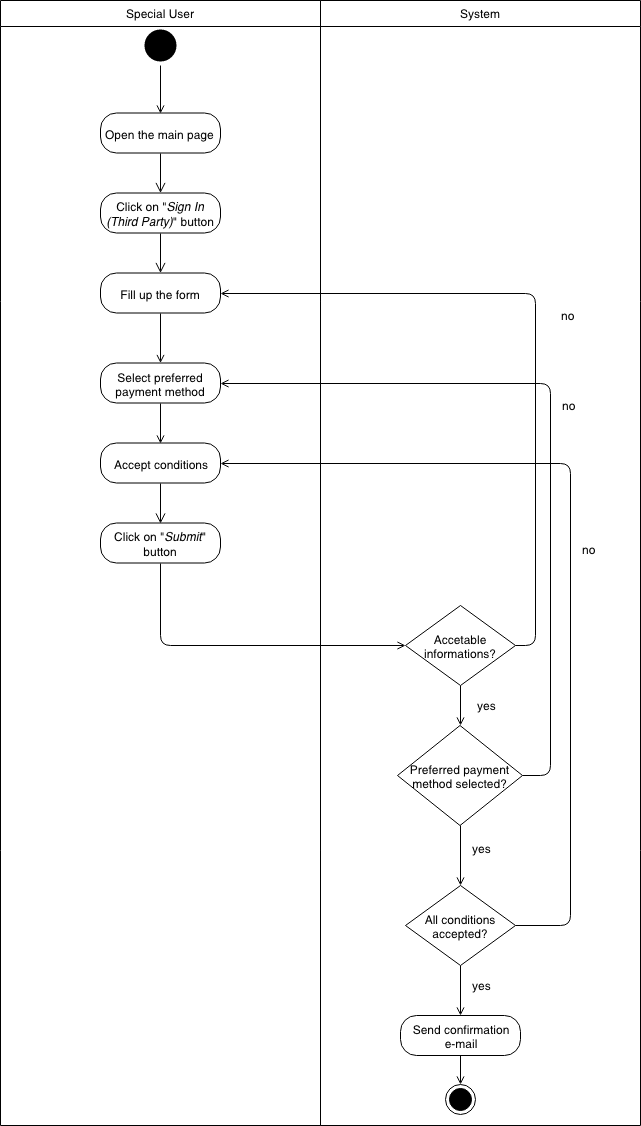
\includegraphics[height=0.6\paperheight]{img/activity/SpecialSignIn.png}
  \hspace{0.05\linewidth}
  \centering
  \caption{\textit{Third Party Sign In} activity diagram}
  \label{img:specialSignInActivityDiagram}
\end{center}
\end{figure}

\begin{figure}[H]
\begin{center}
  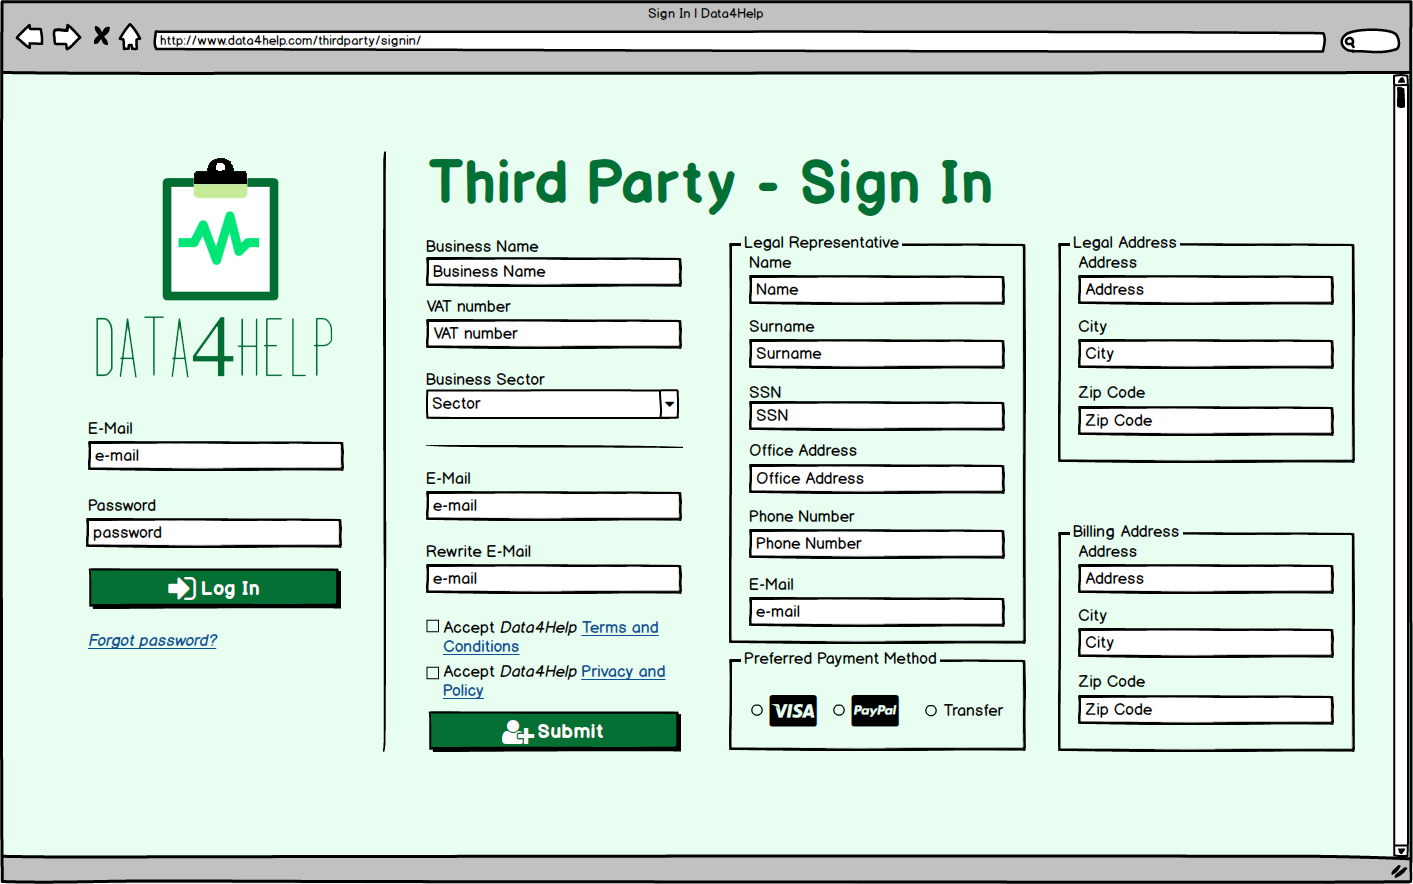
\includegraphics[width=\textwidth]{img/mockup/ThirdParty_SingIn.png}
  \hspace{0.05\linewidth}
  \centering
  \caption{\textit{Third Party Sign In} mockup}
  \label{img:thirdPartySignInMockup}
\end{center}
\end{figure}
